\chapter{Methodology}
\section{Kernel Selection}
So that a breadth of usage scenarios were examined, three kernels were selected based on their conformity to the following set of criteria.
\begin{itemize}
  \item \textbf{The part of the program responsible for more than two thirds of the processing time should not be more than 1500 lines.} To ensure that I fully implemented three ports of existing kernels, it was necessary to limit the size of the kernels that could be considered. This was an unfortunately necessary decision to make. Whilst it reduced the field of possible kernels, it helpfully excluded any overly complex mini-apps.

  \item \textbf{The program must use shared memory parallelism and target the CPU.} Rust's (supposed) zero cost memory safety features are its differentiating factor. The best way to test the true cost of Rust's memory safety features would be through shared memory parallelism, where a poor implementation of memory management will make itself evident through poor performance. Programs which target the GPU rather than the CPU will not be considered, as the current implementations for Rust to target GPUs involve calling out to existing GPU APIs. Therefore, any analysis of a Rust program targeting a GPU would largely be an analysis of the GPU API itself.

  \item \textbf{The program run time should reasonably decrease as the number of threads increases, at least until the number of threads reaches 32.} It is important that any kernel considered is capable of scaling to the high core counts normally seen in HPC.I will be running the kernels on Cirrus, which supports 36 real threads.

  \item \textbf{The program operate on data greater than the CPU's L3 Cache} so that we can be sure that the kernel is representative of working on large data sets. Cirrus has an L3 cache of 45MiB. As each node has 256GB of RAM, a central constraint when working with large data sets is the speed with which data is loaded into the cache. Speed is often achieved by programs in this area through vectorisation, the use of which can be deduced from a program's assembly code. If there is a large performance difference between Rust and the reference kernels, we can use the program's assembly code to reason about that difference.

  \item \textbf{The program must be written in C or C++.} This restriction allows us to choose work which is more representative of HPC programs that actually run on HPC systems, rather than python programs which call out to pre-compiled libraries. Unlike Fortran, C and C++ use array indexing and layout conventions similar to Rust, which will make porting programs from them easier.

  \item \textbf{The program must use OMP.} This is a typical approach for shared memory parallelism in HPC\@. Use of a library to do the parallel processing also further standardises the candidate programs, which will lead to a deeper understanding of the kernel's performance factors.
\end{itemize}

I used this selection criteria to compile a long list of potential kernels to port to Rust. From this long list, I selected the Babel Stream, sparse matrix vector multiplication and K-means clustering.

\subsection{Babel Stream}

Babel Stream is a memory bench marking tool which was developed by the university of Bristol. Babel Stream was written to primarily target GPUs, but it is able to target CPUs too~\cite{BabelStream}.  It is written in C++, supports OpenMP and allows one to set the problem size when executing the program, so we can be sure we exceed the size of L3 cache. My initial tests found the kernel to scale well, and although the program as a whole is quite large, when one ignores parallel technologies excluded by our selection criteria, the amount of code which needs to be ported to Rust falls well within our bounds. I found Babel Stream easy to install and run.

Babel Stream performs simple operations on three arrays of either 32 or 64 bit floating point numbers, $a$, $b$ and $c$. The values of $a$ are set to 0.1, $b$'s to 0.2, and $c$'s to 0.0. Stream performs five operations $n$ times on the arrays, where $n$ is a specified command line argument. The operations are listed below:
\begin{itemize}
  \item \textbf{Copy:} Data is copied from the array $a$ into array $c$
  \item \textbf{Multiply:} Data in $c$ is multiplied by a scalar and stored in $b$
  \item \textbf{Add:} The values in $a$ and $b$ are added together and stored in $c$
  \item \textbf{Triad:} The program then multiplies the new values in $c$ by the same scalar value, adds it to $b$ and stores the value in $a$
  \item \textbf{Dot:} The dot product is performed on arrays $a$ and $b$. This is when every nth element of $a$ is multiplied by the nth element of $b$, and summed.
\end{itemize}
The resulting values in the arrays are then compared against separately calculated reference values, and examined to see if their average error is greater than that number types epsilon value.

Babel Stream's operations are `\textit{memory bandwidth bound}'~\cite{BabelStream}, because they are so simple. Therefore, when implemented through different technologies, Babel Stream provides an insight into the memory bandwidth of that technology, and gives an indication of how the design choices of that technology influences its performance.

\subsection{Sparse Matrix Vector Multiplication}

The Sparse Matrix Vector Multiplication (SpMV) Kernel~\cite{ParResSparse} forms part of the Parallel Research Kernels suite, developed by the Parallel Research Tools group. Sparse matrix vector multiplication (SpMV) is a common HPC operation, used to solve a broad range of scientific problems~\cite{Sedaghati:2015, spMVGPU, DBLP:journals}.

The kernel is mostly one file, sparse.c, which in total is 353 lines of code. The implementation is in C and OpenMP, and my tests found it to scale to a high thread count. As with Babel Stream, the program allows one to set problem size through command line arguments, allowing us to ensure the program operated on data greater than the CPU's L3 cache.

In the selection process, I found that the program's lack of dependencies made it easy to install and run.

The program represents its sparse matrix through the compressed sparse row (CSR) format. This format uses key information about the matrix to avoid storing all of the sparse matrix's redundant zeros in the computer's memory. The information used to do this are the number of rows and columns the matrix has, and the number of non zero values which exist in the matrix. These three values are used to build three vectors, one holding all the non zero values of the matrix, another vector of the same length holding the column indexes for all of those values, in order, and lastly a smaller vector which holds the index at which a particular row starts.

For example, if we wanted the element at 24,32 within the vector, we would look in the 24\textsuperscript{th} element of the row start vector, which would give us the y index of the element. If this did not match the y index we were looking for, in this case 32, we would then look at the next element until we found it. Once we have found the element, we can get the value from the value vector using the index we construct from adding the 24\textsuperscript{th} element of the row start vector, added to however many times we needed to look at the next value to before we found the appropriate y index.

The particular implementation of SpMV which we are porting to Rust uses a user defined grid size, over which a user defined periodic stencil is applied to find the number of non zero entries. The implementation parallelises its initialisation and the actual multiplication of the values using simple \texttt{\#pragma} statements.

This kernel will hopefully provide a realistic idea of how well Rust can perform one of the most common HPC operations.

\subsection{K-Means clustering}

K-means clustering is a `process for partitioning an $N$-dimensional population into $K$ sets'~\cite{macqueen1967}, where the number of sets is less than $N$, and each set of is clustered around a local mean. K-means clustering finds many uses in HPC, particularly in data analysis~\cite{DBLP:journals/corr/ChakrabortyND14a, ordovas2014fast}, and is so ubiquitous throughout HPC that implementations of it are already used to evaluate software and hardware~\cite{Yang2014}.

My reference implementation for this code comes from Jaiwei Zhuang's CS205 project~\cite{CS205}. It is written in C and uses OPENMP, and is less than 200 lines long. The data processed by the program can be generated by a script, allowing me to work on an arbitrary amount of data. The kernel is written so that all processing is done by the CPU\@. It is of particular interest that the kernel reads its data from a NetCDF file, which is common in HPC\@. The code is well documented and concise.

After the Kernel has read in the program data, it performs the clustering process. It does this by first filling the \texttt{old\_cluster\_centres} array with random data, and then beginning its central processing loop.\todo{add more info on variables purposes here}
\begin{itemize}
  \item \textbf{Expectation:} Assign population points to their nearest cluster centre, by looping over every member of the population, and finding the minimum distance between that point all the cluster centres. This is the stage which is parallelised.
  \item \textbf{Maximisation:} Next, the cluster centres are set to the mean, which is calculated in two steps.
  \begin{itemize}
    \item \textbf{1:} The size of the cluster is calculated by looping over every point and finding its cluster centre, and then incriminating that cluster centres population count. The sum of the points in that cluster is also calculated and stored in the \texttt{new\_cluster\_centres} array.
   \item \textbf{2:} The sum of the cluster is divided by the size of it, and stored in to the \texttt{old\_cluster\_centres} for use on the next iteration of the loop.
   \end{itemize}
\end{itemize}
This loop continues until it reaches a pre-defined maximum iteration value, or the sum of the minimum distance values becomes less than a certain tolerance value. The program then writes data back out to the NetCDF file it read the data from originally.

I found this program quite difficult to install and run due to the NetCDF dependency. My first attempt to install NetCDF through the script included in the repository ended with me unable to boot into my laptop. Subsequent attempts to install NetCDF through package managers were also not successful, although they were less damaging to my system. To compile the kernel on Cirrus I had to make sure I had selected the correct combination of NetCDF and HDF5 library versions, mostly through guess work. However, once I had accomplished this task, compiling the program itself was easy. The kernel then showed itself to be able to scale well enough for the interests of this project.
\section{Implementation}
Implementation of all three programs followed the same process, as outlined in Figure~\ref{fig:imp-flow}. The full process would take between three to four weeks to complete for each kernel. I first implemented Babel Stream, then the sparse matrix multiplication kernel and finally the K-means kernel, in that order.

\begin{figure}
  \center
  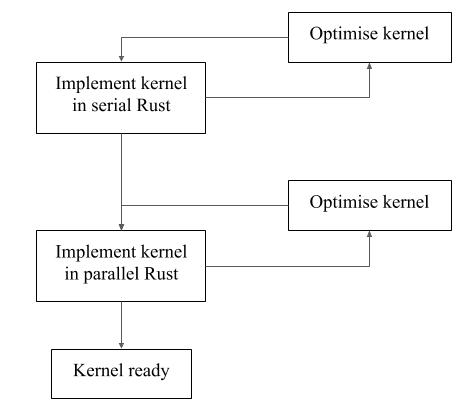
\includegraphics[height=8cm]{figs/ImplementationFlow.png}
  \caption{Flow diagram for implementation process}
  \label{fig:imp-flow}
\end{figure}

\subsection{Porting to Serial Rust}
Once a candidate kernel is selected, it is implemented in Rust in serial. Any differences between the  behaviour of the Rust and the original implementation are thought of as bugs, and are eradicated or minimised as far as is possible. For ease of development, the Rust crate Clap~\cite{RustClap} was used to read command line arguments for the program, leading to Rust implementations of kernels being called with slightly different syntax. This difference was deemed to be superficial enough to be allowable. Kernel output was as similar as possible to aid data-collection from both implementations.

Babel Stream was in some ways one of the hardest to Kernels to port to serial Rust. This was partly due to it being the first program which I attempted to port, but also because of Rust's type system and the use of generics. The original C++ implementation of the program uses templates to allow the user to choose to use 32 or 64 bit floating numbers when running the program. To achieve the same thing in Rust, generic types have to be used, which are defined through traits.

I found that using generics in Rust made reading error messages difficult, but easier to parse once the offending code was removed into a smaller example, and stripped of its generic type. Generics in Rust necessitate slightly cumbersome syntax, for example, \texttt{T::from(0).unwrap()} is used to generate a zero of type T. The first part of this expression generates an option type, which in this case is \texttt{Some(0.0)}, and is then unwrapped into simply \texttt{0.0}. Rust does this to allow programmers to deal with cases where a value of type T is impossible to generate from the input value, such as casting a value greater than $2^{32} - 1$ to a signed 32 bit value. In this circumstance, the value returned would be \texttt{None}, which the programmer would then have to deal with. As zero can always be successfully cast to a 32 or 64 bit floating point number, it is safe to simply unwrap the value here, but if it was a number that could not be cast to the type, then the program would crash at this point. A C or C++ program doing the same thing would not crash, but its result would be implementation specific undefined behavior, or throw an exception. \todo{should I discuss the design choices made here, and their implications for Rust in HPC}

The Rust implementation of Babel stream, like the reference implementation, creates a stream object which calls certain functions on its own data sets. This was quite easy to implement as Rust has enough features of object oriented programming, such as allowing objects to contain data and behaviour, for these simple objects to work. However, Rust does not implement inheritance, which is considered by some to be a foundational aspect of object oriented programming~\cite{Liskov:1987}, and instead uses trait objects to share behaviours. This design choice did not interfere with any of the simple kernels which were implemented, but would certainly be interesting to translate object inheritance from a larger program, maybe a mini-app, into Rust's trait feature.

Whilst the concept of borrowing did take some time to fully understand, I found that the compiler gave very helpful and accurate hints on how to make sure my program complied with the borrow checker. For example, in listing~\ref{lst:comp-help}, the programmer is informed that they `cannot borrow self.c as mutable', and is shown where the function tries to mutate the value. The stream object's triad function, which alters the objects data, but take mutable ownership of the data, through using \texttt{\&mut self}, where \texttt{\&mut} is a mutable borrow. Once the programmer implements the compiler's suggested fix, this fragment of code will compile.

\begin{alltt}
\scriptsize
error[E0596]: cannot borrow `self.c` as mutable, as it is behind a
              `&` reference
  --> src/stream.rs:20:9
   |
18 |     pub fn triad(&self)\{
   |                  ----- help: consider changing this to be a
    mutable reference: `&mut self`
20 |         self.c[0] = self.a[0] + self.b[0];
   |         ^^^^^^ `self` is a `&` reference, so the data it refers
    to cannot be borrowed as mutable
error: aborting due to previous error
\end{alltt}

The sparse matrix vector multiplication kernel was quite simple to port to serial Rust, as I was able to ignore parts of the small program which would not be used. As with Babel Stream, I found converting from C's data types into Rust to be a stumbling point due to Rust's safety constraints. For example, in the C implementation, the vector holding the column index of the matrix was composed of values of type \texttt{s64Int}, which a signed 64 bit int. This datatype is directly analogous to Rust's \texttt{i64} data type, except in C you may use numbers of type \texttt{s64Int} to index into arrays, where as in Rust you must only use numbers of type \texttt{usize}. Errors of this type are easily dealt with however, as they are explicitly pointed out to the programmer at compile time, and can be remedied with casts in the simple format \texttt{as usize}. I found sparse matrix vector multiplication easier to port to serial Rust than Babel Stream, but this could have been that by this point I was already more familiar with Rust's way of doing things.

Given the difficulty I had trying to install the dependencies for the reference implementation of the K-means clustering Kernel, it was surprisingly easy to get NetCDF working with Rust. I simply found a NetCDF rust library~\cite{RustNetCDF}, which I added to my implementation's \texttt{Cargo.toml} file. I was then able to easily compile and use this library within my K-means implementation.

An interesting factor in writing the K-Means cluster in Rust was porting the original helper functions, which were used to make 2d integer and 2d float arrays. In the original C implementation, these 2d arrays were \texttt{float**} and \texttt{int**}. When I was porting these data structures to Rust, it was important to consider if data locality impacted their use. The original implementation used the data a column wise operation, so that the next datum to be used was likely to have already been loaded in the same cache line as the previous one. This allowed me to write my implementation as a vector of \texttt{f32} or \texttt{i32} vectors.

The Rust vector of vectors was generated from a single one dimensional vector using the same algorithm as the reference implementation, where sections of the original vector are read into the new vectors within the vector of vectors. Although the original is well suited to C's memory management idioms, it was easy to write the same method in safe rust. The ease with which I was able to re-implement this routine is another suggestion of Rust's ability to replace C's use in HPC.

\subsection{Serial Optimisation}
Next, I eliminated any bugs found in my serial implementation of the code by comparing outputs between my implementation and the reference implementation. During this process I would also move the code away from its C style towards more idiomatic Rust. To achieve more idiomatic Rust, I used the linting tool Clippy~\cite{RustClippy}, which was developed by the Rust team.  Clippy includes a category of lints  which highlight `code that should be written in a more idiomatic way'~\cite{RustClippy}. I implemented all of Clippy's recommended rewrites, which would often include replacing the use of for loops over integer indexes to access vector variables with calls to the vector's \texttt{iter()} method. This particular replacement requires code to be rewritten in a much more functional style.

For example, all of the array operations in Babel Stream where originally written in a C style, and then transformed to use iterators. Listing~\ref{lst:iters-b}, shows the original, more succinct for loop form of Babel Stream's add operation. This style is rejected by Clippy, which prefers the style presented by listing~\ref{lst:iters-a}.

\noindent\begin{minipage}{.45\textwidth}
    \begin{code}
\begin{minted}{rust}
for i in 0..self.c.len() as usize {
    self.c[i] = self.b[i] + self.a[i]
}
\end{minted}
\captionof{listing}{Babel Stream Add, before applying idiomatic Rust style}
    \label{lst:iters-b}
\end{code}
\end{minipage}\hfill
\begin{minipage}{.45\textwidth}
    \begin{code}
\begin{minted}[fontsize=\scriptsize]{rust}
for ((c, b), a) in self.c.iter_mut()
                 .zip(self.b.iter())
                 .zip(self.a.iter()){
    *c = *b + *a;
}
\end{minted}
\captionof{listing}{Babel Stream Add, after applying idiomatic Rust style}
\label{lst:iters-a}
\end{code}
\end{minipage}

Whilst the more idiomatic rust style in listing~\ref{lst:iters-a} is less succinct than~\ref{lst:iters-b}, it does have some benefits which the C style for loop does not possess. For example, if the stream object's c array had been of greater length than its $a$ or $b$ arrays, the more C-like implementation would fail at run time with an index out of bounds error, whereas the more idiomatic code only write to as many elements of $c$ as the least elements there are of any of the arrays it is zipped with.

Also note in listing~\ref{lst:iters-a} the distinction between the methods \texttt{iter()} and \texttt{iter\_mut()}, the first of which creates an iterator, and the second of which creates an iterator which may change its elements. Although an in-depth investigation was not carried out to see if the compiler made use of any optimisations here from the greater amount of information available to it, the time to run this fragment did decrease when converted to idiomatic Rust, from 0.09501 seconds to 0.09079 seconds.

A bug in my SpMV implementation was found at this stage. When launched with certain parameters, the C version ran without error, whilst the Rust version would panic and fail every time, with the error message:

\begin{alltt}
\scriptsize
thread `main' panicked at `attempt to shift left with overflow', main.rs:8:13
\end{alltt}

It became apparent that this was occurring because although I had mirrored the types used by the reference implementation, the behaviour of those types differed. In the reference implementation, radius was of type \texttt{int}, which is a 32-bit integer. I therefore translated this into a \texttt{i32} type in Rust. These values are used as upper limits in an initialisation loop, where intermediate values of the same type are bit-shifted before being stored in the colIndex array. In C, the operation shown in the listing~\ref{lst:bit-shift} sets $foo$ to 2, when all numbers are 32 bit integers. 

\begin{code}
\begin{minted}{c}
int foo = 1 << 33;
\end{minted}
\captionof{listing}{Bit shift overflow in C}
\label{lst:bit-shift}
\end{code}

This occurs because the value 1 overflows and rolls over. In Rust however, this code causes the program to panic and quit~\footnote{The compiler will catch this error before run time if it can calculate the value 1 will be shifted by}. The Rust language does not consider this behaviour to be unsafe, but finds that that the programmer `should' find it `undesirable, unexpected or unsafe'~\cite{rustunsafe}. However, Rust does recognise that some programs do rely upon overflow arithmetic, and provides mechanisms to enable this feature in the language. Fortunately, I was not required to use this feature after changing radius from the \texttt{i32} type to \texttt{usize} type, which is 64 bits. This choice was made because the radius values were being cast to \texttt{usize} more often than they were being used as \texttt{i32}. This had the consequence of making the program impossible to bit shift overflow, as a radius of 64 requires a stencil diameter greater than $2^{32}-1$, which would in turn require a colindex array terabytes in size, which the Cirrus hardware does not support.

When this optimisation pass was applied to K-means, it showed the limits of Clippy's linter. Clippy flagged concise for loops with warnings, and suggested overly verbose rewrites of them. For example, on line 110 of the kernel, just before the second part of the maximisation is about to begin, Clippy complains that listing~\ref{lst:for-concise} has a `needless range loop'.

\begin{code}
\begin{minted}{rust}
for k in 1..clusters_d.len as usize {
\end{minted}
\captionof{listing}{Needless range loop}
\label{lst:for-concise}
\end{code}
Clippy argues this pattern should be avoided, because `iterating the collection itself makes the intent more clear and is probably faster'~\cite{ClippyLoop}. However, its suggested replacement is much longer, and the deeply chained methods take longer to comprehend.
\begin{code}
\begin{minted}{rust}
for (k, <item>) in old_cluster_centres.iter()
                                       .enumerate()
                                       .take(clusters_d.len as usize)
                                       .skip(1) {
\end{minted}
\captionof{listing}{Clippy's suggested iterator}
\end{code}
It would be difficult to argue that the code suggested by Clippy is idiomatic, as idiomatic code is generally agreed to be code which uses features of the language to achieve conciseness. This code fragment is clearly not concise, and I therefore did not make Clippy's suggested correction.
\subsection{Parallelisation}
I then parallelised the kernel with Rayon~\cite{RustRayon}, at the same loops where the reference implementation uses OpenMP\@. Sometimes this would be a simple matter of replacing the \texttt{iter()} method with \texttt{par\_iter()}, but parallising more complex operations like reductions and initialisation was slightly more difficult.

Parallelising Babel Stream was simple. As listing~\ref{lst:iters-p} shows, Babel Stream's add operation remains largely the same, only that the \texttt{iter()} method has been replaced by the \texttt{par\_iter()} method, and that the method for each has to be called. As the serial version of this loop had no inter loop dependencies, it coud easily be transformed from a for loop to a parallel for each loop.
\begin{code}

\label{lst:iters-p}
\begin{minted}[fontsize=\scriptsize]{rust}
self.c.par_iter_mut()
            .zip(self.b.par_iter())
            .zip(self.a.par_iter())
            .for_each(|((c, b), a)| *c = *a + *b);
\end{minted}
\captionof{listing}{Babel Stream Add, parallelised}
\end{code}

This pattern was applicable to the copy, multiply, add, and triad methods. The dot method needed more alteration than these methods to be parallelised, as the original, Clippy compliant code was very different to the final code used. The original code in Listing~\ref{lst:dot-for} updates the sum value from within a for loop before returning it.
\begin{code}
\begin{minted}[fontsize=\scriptsize]{rust}
let mut sum1: T = T::from(0).unwrap();
for (a, b) in self.a.iter()
                    .zip(self.b.iter()){
                      sum1 += a * b;
                    }
sum1
\end{minted}
\captionof{listing}{Serial Dot Product}
\label{lst:dot-for}
\end{code}
This update pattern does not work with a Rayon parallel for each loop, as threads are not able to write to a shared variable. The Rust compiler gives the error that the closure does not implement \texttt{FnMut}, which is `The version of the call operator that takes a mutable receiver'~\cite{rust-doc-fnmut}. A mutable receiver in this case refers to a mutable variable which is created, and lives on, outside of the iterator's scope. This error demonstrates the utility of Rust's mutable and immutable variables in parallel operations.

To solve this error, the expression is rewritten using the fold method. It was quite difficult to find how to exactly write this, as the serial fold method has a different call signature to the Rayon parallel fold. The final implementation of Babel Stream's fold is shown in Listing~\ref{lst:dot-fold}.
\begin{code}
\begin{minted}[fontsize=\scriptsize]{rust}
let sum1: T = T::from(0).unwrap();
self.a.par_iter()
    .zip(self.b.par_iter())
    .fold(|| sum1, |acc, it| acc + *it.0 * *it.1).sum()
\end{minted}
\captionof{listing}{Parallel dot product}
\label{lst:dot-fold}
\end{code}
In this listing, a zero of type T is generated, and the vectors a and b are zipped together, as before. The fold method then takes two arguments, both of which are closures, or anonymous functions. The first closure is used to create the identity value, which is the value which can be used as the initial accumulator value when the zipped vector of \texttt{a} and \texttt{b} is divided between threads. The zipped vector of \texttt{a} and \texttt{b} takes the form

\begin{center}
$[(a_1, b_1), (a_2, b_2), \ldots, (a_{n-1}, b_{n-1})]$
\end{center}

The fold is applied, resulting in the form:

\begin{center}
$[a_1b_1, a_2b_2, \ldots, a_{n-1}b_{n-1}]$
\end{center}
Which is reduced to the a single number, through calling \texttt{sum()}

\begin{center}
$a_1b_1+a_2b_2+\cdots+a_{n-1}b_{n-1}$
\end{center}

Although the initial change of perspective required to use Rayon's fold was confusing, once the cognitive leap had been made the simplicity was clear. Although it was hard to use Rayon's fold method, I did not find it to be prohibitively difficult.

Most of the methods of Babel Stream were easy to parallelise, but this does not necessarily show us the expressiveness of the Rayon library. The parallelised methods were so simple that they were extremely unrepresentative of production HPC code. The sparse matrix vector multiplication parallelisation was more representative of the type of parallelism which is done in HPC, and was therefore more complex than babel stream. Even so, parallelising the central processing loop of SpMV was trivial.
\noindent\begin{minipage}{.48\textwidth}
\begin{code}
\begin{minted}[fontsize=\scriptsize]{rust}
for row in 0..size2 as usize {
  let first = stencil_size * row;
  ...
  result[row] += temp;
}
\end{minted}
\captionof{listing}{Serial SpMV}
\end{code}
\end{minipage}\hfill
\begin{minipage}{.48\textwidth}
\begin{code}
\begin{minted}[fontsize=\scriptsize]{rust}
result.par_iter_mut()
      .enumerate()
      .for_each( |(row, item)| {
  let first = stencil_size * row;
  ...
  *item += temp;
}
\end{minted}
\label{lst:spmv-par}
\captionof{listing}{Parallel SpMV}
\end{code}
\end{minipage}

In the parallel version of the spare matrix vector multiplication I created a parallel mutable iterator over the result vector, and enumerated it. This allowed me to access the items and the indexes of the vector, which I used without changing the internal logic of the for loop at all. The applicability of this common HPC pattern from C into Rust indicates that Rust is an expressive language for HPC.

The K-means kernel's Expectation stage, or E-step, was harder to parallelise. This difficulty arose from trying to do two, seemingly mutually exclusive things, within the same loop. The code required me to update the values of the array and perform a reduction on another variable external to the loop. I had encountered the difficulty of reducing to a shared variable from multiple threads before, with Babel Stream's dot product (see Listing~\ref{lst:dot-fold}), but was unaware of how to perform this reduction with side effects.

After some experimentation, I found the solution, a simple \texttt{map()} and then \texttt{sum()}. 

\begin{minipage}{.48\textwidth}
\begin{code}
\begin{minted}[fontsize=\scriptsize, frame=single]{rust}
for (idx, item) in x.iter()
                    .enumerate(){
    ...
    labels[idx] = k_best;
    dist_sum_new += dist_min;
}
\end{minted}
\captionof{listing}{K-means Rust serial E-step}
\label{lst:kmeansserial}
\end{code}
\end{minipage}\hfill
\begin{minipage}{.48\textwidth}
\begin{code}
\begin{minted}[fontsize=\scriptsize, frame=single]{rust}
dist_sum_new = labels.par_iter_mut()
                .enumerate()
                .map(|(idx, item)| {
    item = k_best;
    dist_min
    }).sum();
\end{minted}
\captionof{listing}{K-means Rust parallel E-step}
\label{lst:kmeanspar}
\end{code}
\end{minipage}

In Listing~\ref{lst:kmeansserial} I am creating an iterator over \texttt{x}, which is a vector of the length as the vector \texttt{labels}. I had originally chosen this vector to be the one which created the iterator merely for convenience. I had to change this vector to \texttt{labels} in the parallel implementation however, as it is the items of \texttt{labels} that need to be updated. I then used the index value to retrieve the necessary values from \texttt{x} to calculate the value of \texttt{k\_best}. The value of \texttt{dist\_min} is also calculated for that particular index value. These \texttt{dist\_min} values are left in a map structure, which is reduced by the sum and written to \texttt{dist\_sum\_new}, yielding the same result as the serial implementation. 

\todo{reflection on this use pattern}


\subsection{Parallel Optimisation}
Once I had parallelised the Rust implementations, I carried out another optimisation pass. This optimisation pass allowed me to find issues caused by parallelism, and make improvements only possible through parallelism. One such improvement was parallel initialisation.

Parallel initialisation is an important feature of programs which run on cache coherent non uniform memory address (CC-NUMA) systems. CC-NUMA systems often use a first touch allocation policy, which means that the each memory address that is written to, or page, is located near to the processor which first touched it. The 18 core Intel Xeon processors on Cirrus use this particular memory allocation policy, which therefore means that `poorly written applications (e.g., initializations  performed  at  a  single  processor  before  main  parallel computation  begins)  will  locate  pages  incorrectly based  on  the  first  access  and  cause  several  remote memory accesses later'~\cite{Bhuyan:2000}. Without parallel initialisation, the Rust implementation of Babel Stream falls under this definition of a poorly written application. Preliminary testing had also found that the Rust implementation's performance had failed to scale past 8 threads, whilst the C++ implementation's performance continued to increase up to 24 threads. 

I had not yet prioritised written parallel initialisation in Rust as there was no clear way to do it. This was largely because in the C++ form of parallel initialisation, allocating the memory to be used and then initialising that memory are two distinct steps, where as in Rust they are the same step.

\noindent\begin{minipage}{.48\textwidth}
\begin{code}
\begin{minted}{c}
#pragma omp parallel for
for (int i = 0; i < array_size; i++)
{
    a[i] = initA;
    b[i] = initB;
    c[i] = initC;
}
\end{minted}
\label{lst:serialInit}
\captionof{listing}{Babel Stream C parallel initilisation}
\end{code}
\end{minipage}\hfill
\begin{minipage}{.48\textwidth}
\begin{code}
\begin{minted}{rust}
vec![0.0; arr_size].par_iter()
       .map(|_| T::from(0.2).unwrap())
       .collect_into_vec(&mut self.b);
\end{minted}
\label{lst:parInit}
\captionof{listing}{Babel Stream Rust parallel initilisation}
\end{code}
\end{minipage}

Listing~\ref{lst:serialInit} shows how the C++ version of Babel Stream carries out its first touch in parallel, by adding a simple \texttt{\#pragma} statement to the code. This pattern is not reproducible with Rayon, as it doesn't use parallel for loops, but instead uses parallel iterators. The solution was found to be using the map function to collect values into a vector, as shown in listing~\ref{lst:parInit}.

This routine works by using the \texttt{vec!} macro to create a vector of length \texttt{arr\_size}, where every value in the vector is 0.0. This vector is then used to generate a parallel iterator. The parallel iterator performs a map, taking all values from the vector, and generating a corresponding 0.2, of type T. The \texttt{|\_|} notation here means that although the closure signature requires a value, that value will not be used in the closure's method.
These values of 0.2 are then collected into the vector held in \texttt{self.b}.

The use of map here to generate values for parallel initialisation seems like it is an unlikely use case scenario, but I discovered how to use it from the rayon documentation on the map method~\cite{rayonMap}. Whilst clear documentation always helps a language to become more accepted, this use case was shown to not be as flexible as was needed by all kernels which were ported to Rust, as was found later when attempting to implement parallel initialisation for SpMV.

\begin{figure}[h]
    \centering
    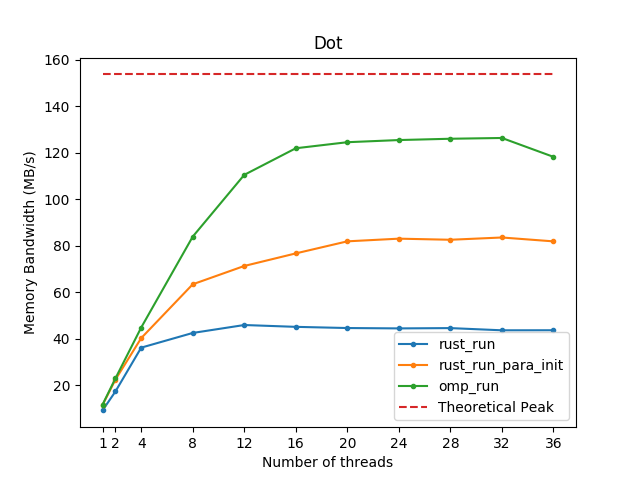
\includegraphics[width=.8\linewidth]{figs/babel/dot-init.png}
    \caption{Babel Stream Memory Bandwidth initialisation comparison}
    \label{fig:babel-dot-init}
\end{figure}

Figure~\ref{fig:babel-dot-init} shows, the use of parallel initialisation greatly improved the memory bandwidth of the Babel Stream. However, the improvement in performance still did not bring it to a parity with the C++ and OMP implementation, for reasons discussed further in section~\ref{sec:res-babel}.

The initilisation routine for the Sparse Matrix Vector Multiplication kernel was not as easy to implement. The difficulty was that the parallel loop used to write to elements of the vector \texttt{colIndex}, wrote to the vector in chunks of five. This made it very hard to translate into Rust, as Rayon only uses parallel iterators, and has no exact equivelent of parallel for loops.

Within an iterator, the programmer may only access the current element of the array, and the next element of the array. This restricted functionality is not expressive enough for the initilisation routine shown in listing~\ref{lst:sparseParaInit}, as we are unable to step in fours, and we are unable to access the next element of the vector without starting the iterator routine from it's first instruction again.


\begin{code}
\begin{minted}{c}
#pragma omp for private (i,j,r)
for (row=0; row<size2; row++) {
j = row/size; i=row%size;
elm = row*stencil_size;
colIndex[elm] = REVERSE(LIN(i,j),lsize2);
    for (r=1; r<=radius; r++, elm+=4) {
      colIndex[elm+1] = REVERSE(LIN((i+r)%size,j),lsize2);
      colIndex[elm+2] = REVERSE(LIN((i-r+size)%size,j),lsize2);
      colIndex[elm+3] = REVERSE(LIN(i,(j+r)%size),lsize2);
      colIndex[elm+4] = REVERSE(LIN(i,(j-r+size)%size),lsize2);
    }
...
}
\end{minted}
\captionof{listing}{SpMV C Parallel Initilisation}
\label{lst:sparseParaInit}
\end{code}

Several methods were used in an attempt to solve this problem, including creating an object which would have permanance between iterations. However, this method was unsuccseful as the rayon iterator's did not implement \texttt{FnMut}. This problem was ultimitely solved using Rust's parallel primitives:

\begin{itemize}
    \item \texttt{Mutex} - Protects shared data through mutual exclusion of locks.
    \item \texttt{channel} - Used to send data between threads.
    \item \texttt{Arc} - An atomic reference counter, which provides shared ownership of a value between threads.
    \item \texttt{thread} - The most basic threading model available in Rust. Platform agnostic.
\end{itemize}

These primitives were then used to initilise the \texttt{col\_index} array thusly.

\begin{enumerate}
    \item The main thread creates a vector, and wraps it in a \texttt{Mutex} which is wrapped in an \texttt{Arc}, which is labelled \texttt{col\_index}
    \item The main thread uses the \texttt{channel} to create a sender and a receiver nodes.
    \item The main thread enters a loop, where it creates clones of the n threads worth of \texttt{col\_index} constructs and sender nodes, which it then moves into spawned threads. Each thread is given a consecutive thread ID starting from 0.
    \item Each thread calculates the section of \texttt{col\_index} it will write to from its thread ID and the size of the overall \texttt{col\_index}. This section is called \texttt{my\_col\_index}, and is created as a vector of zeros of the correct length for that thread and filled with zeros, which are then overwritten according to the original algorithm.
    \item Each thread then attempts to aquire the lock for the shared \texttt{col\_index}, and checks the length of it.
    \begin{enumerate}
        \item If the length of \texttt{col\_index} is the same as the lower bound of that thread's section, then the thread appends its \texttt{my\_col\_index} to \texttt{col\_index}, which it then releases the lock for.
        \item Otherwise, the releases the lock and periodically re-acquires it until \texttt{col\_index} is the right length.
    \end{enumerate}
\item Once the last thread has appeneded their \texttt{my\_col\_index} to \texttt{col\_index}, it sends an empty message to the master thread.
\item The master thread, which has been blocking, receives this message, and joins all the child threads. It then aquires the lock for \texttt{col\_index} and unwraps it, so that it can now be used as a normal vector.
\end{enumerate}

This whole routine is 62 lines of code, which is more than four times the original 16 lines of code. It was hard to find this solution, as requiring threads to operate in a specific order is not a typical use case scenario. 
The solution is complex, and brittle. Its verbosity makes it harder to read than the original code, and the need for careful array calculations feels unfaithful to the Rust philosophy of safety.

When implementing this solution, I kept running into array index out of bounds errors, implying that I was trying to write outside the array boundaries. These errors would crash the program. The cause of this issue was traced to the original implementation of the program, in C. I found this error by checking the final index written to by the threads, which was two more than the length of the array, if the program was run with certain input parameters. This error goes unnoticed in the C version of SpMV, because whilst a write overrun of 16 bits can cause a program to crash, on a modern system like Cirrus it is unlikely to. I corrected my program's threads to write only within the boundaries of their vectors, and filed an issue for this bug on the ParRes Kernels' github repository~\cite{SparseBug}.

Despite the negatives of the Rust version of the parallel initilisation, it did not have any bugs. Figure~\ref{fig:sparse-speedup} shows the benefit of implementing parallel initilisation for SpMV, which gives the Rust version better scaling than the C version, although its final speed is still slower than the C version's final speed. This difference will be discussed in more detail in section~\ref{sec:res-sparse}

\begin{figure}[h]
    \centering
    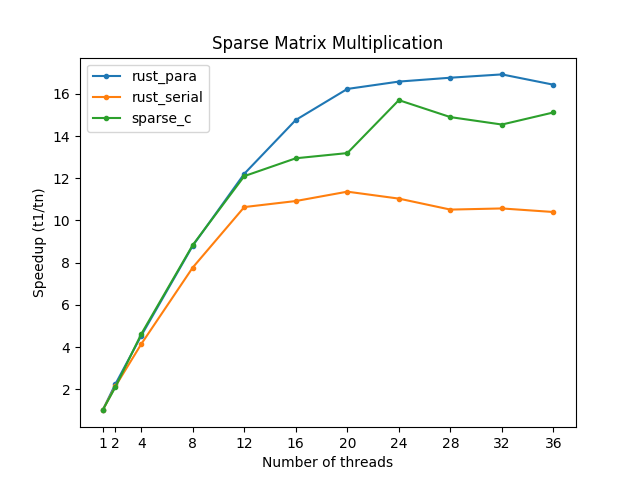
\includegraphics[width=.8\linewidth]{figs/sparse/speedup.png}
    \caption{SpMV speed up comparison}
    \label{fig:sparse-speedup}
\end{figure}

The K-means kernel did not use any parallel initlisation, and therefore did not undergo parallel optimisation.

\section{Experimentation}
All experiments were run on a single node of Cirrus. No other users had access to that node whilst experiments were being run. Each node on cirrues has 36 cores, spread across two 18 core Intel Xeon processors. Each processor shares a 45MiB L3 cache between its 18 cores, with smaller L1 and L2 caches for each individual core.Each processor belongs to a seperate NUMA region, leading to increased latency when retrievinng data from the other NUMA region~\cite{CirrusHardware}.

To reduce the impact of anamolous runs, both versions of each Kernel were run for 100 iterations, and the average speed was taken. Experiments were submitted to cirrus through the use of Portable Batch Script (PBS) files, which returned program output to timestamped files. A sample PBS submission file can be found in Appendix~\ref{app:launch}.
\section{Questionnaire}
To further assess the suitability of Rust for HPC, I presented staff and students at Edinburgh's Parallel Computing Centre (EPCC) with a questionnaire. The aim of this questionnaire was to examine how easily people with little to no experience of Rust could understand it. The more understandable a language is, the easier it is to learn, the more likely it is to be adopted. This questionnaire would provide valuable data on the usability of Rust as a language.

The Questionnaire was formed of seven multiple choice questions, designed to test the participant's knowledge of Rust. An eighth question was also given, which asked the participant how skilled they were at various programming languages.
To minimise the factors of impostor syndrome~\cite{langford1993} and the Dunning-Kruger effect~\cite{kruger1999}

A copy of the questionnaire can be found in Appendix~\ref{app:quest}
